\documentclass[border=6pt]{standalone}
\usepackage[scaled]{helvet}
\renewcommand\familydefault{\sfdefault}
\usepackage{amsmath}
\usepackage{tikz}
\usetikzlibrary{arrows.meta, calc, shapes.arrows, positioning}

% ---------------- colours ----------------
\definecolor{blueFill}{HTML}{BDD4F2}
\definecolor{blueLine}{HTML}{1F4E89}
\definecolor{bluePanel}{HTML}{E4EEFB}
\definecolor{blueDark}{HTML}{163A66}
\definecolor{grayFill}{HTML}{DCE1E7}
\definecolor{grayLine}{HTML}{5D6D7E}
\definecolor{grayDark}{HTML}{3E4A57}
\definecolor{orangeFill}{HTML}{E8710A}
\definecolor{orangePanel}{HTML}{FDE8D5}
\definecolor{orangeLine}{HTML}{C25E06}
\definecolor{greenFill}{HTML}{C8EBD2}
\definecolor{greenLine}{HTML}{1E8449}
\definecolor{docFill}{HTML}{BDD4F2}
\definecolor{docLine}{HTML}{1F4E89}
\definecolor{embBlue}{HTML}{1F4E89}
\definecolor{embOrange}{HTML}{E8710A}
\definecolor{titleColor}{HTML}{163A66}
\definecolor{chevColor}{HTML}{8A9BB0}

\tikzset{
  stagetitle/.style={font=\large\bfseries, align=center, text=titleColor},
  box/.style={draw=#1, rounded corners=4pt, line width=0.7pt, align=center, font=\small\bfseries},
  tag/.style={draw=grayLine, fill=white, line width=0.5pt, minimum width=1.55cm,
              minimum height=0.68cm, align=center, font=\scriptsize\bfseries, inner sep=1pt},
  arr/.style={-{Stealth[length=2.2mm]}, line width=0.7pt, color=grayDark},
  edge/.style={-{Stealth[length=1.6mm]}, line width=0.45pt, color=grayDark!85},
  chevron/.style={single arrow, fill=chevColor, draw=none, minimum width=0.95cm,
                  minimum height=0.85cm, single arrow head extend=0.18cm},
  lbl/.style={font=\small\bfseries, align=center},
}

% ---------------- icons ----------------
% document: \docicon{x}{y}
\newcommand{\docicon}[2]{%
  \begin{scope}[shift={(#1,#2)}]
    \draw[docLine, fill=docFill, line width=0.6pt]
      (-0.5,-0.65) -- (0.5,-0.65) -- (0.5,0.42) -- (0.27,0.65) -- (-0.5,0.65) -- cycle;
    \draw[docLine, fill=white, line width=0.6pt] (0.27,0.65) -- (0.27,0.42) -- (0.5,0.42);
    \foreach \y in {0.28,0.08,-0.12,-0.32,-0.5}
      \draw[docLine, line width=0.9pt] (-0.34,\y) -- (0.32,\y);
  \end{scope}}
% building: \buildingicon{x}{y}
\newcommand{\buildingicon}[2]{%
  \begin{scope}[shift={(#1,#2)}]
    \fill[grayLine] (-0.75,-0.9) rectangle (0.25,0.95);
    \fill[grayLine!70] (0.25,-0.9) rectangle (0.95,0.25);
    \fill[grayLine!70] (-1.2,-0.9) rectangle (-0.75,-0.05);
    \foreach \i in {0,1,2} \foreach \j in {0,...,5}
      \fill[white] ({-0.63+\i*0.3},{-0.5+\j*0.235}) rectangle ++(0.17,0.13);
    \foreach \i in {0,1} \foreach \j in {0,1,2}
      \fill[white] ({0.38+\i*0.27},{-0.5+\j*0.24}) rectangle ++(0.14,0.13);
    \foreach \j in {0,1}
      \fill[white] (-1.07,{-0.5+\j*0.24}) rectangle ++(0.17,0.13);
    \fill[white] (-0.36,-0.9) rectangle (-0.14,-0.62);
    \draw[grayLine, line width=1pt] (-1.35,-0.9) -- (1.1,-0.9);
  \end{scope}}
% embedding bar: \embbar{x}{y}
\newcommand{\embbar}[2]{%
  \foreach \k/\c in {0/embBlue,1/embBlue,2/embOrange,3/embBlue,4/embOrange,5/embOrange,6/embBlue,7/embOrange}
    \draw[white, line width=0.4pt, fill=\c] ({#1+\k*0.2},{#2-0.11}) rectangle ++(0.2,0.22);
  \draw[grayDark, line width=0.4pt] ({#1},{#2-0.11}) rectangle ++(1.6,0.22);}

\begin{document}
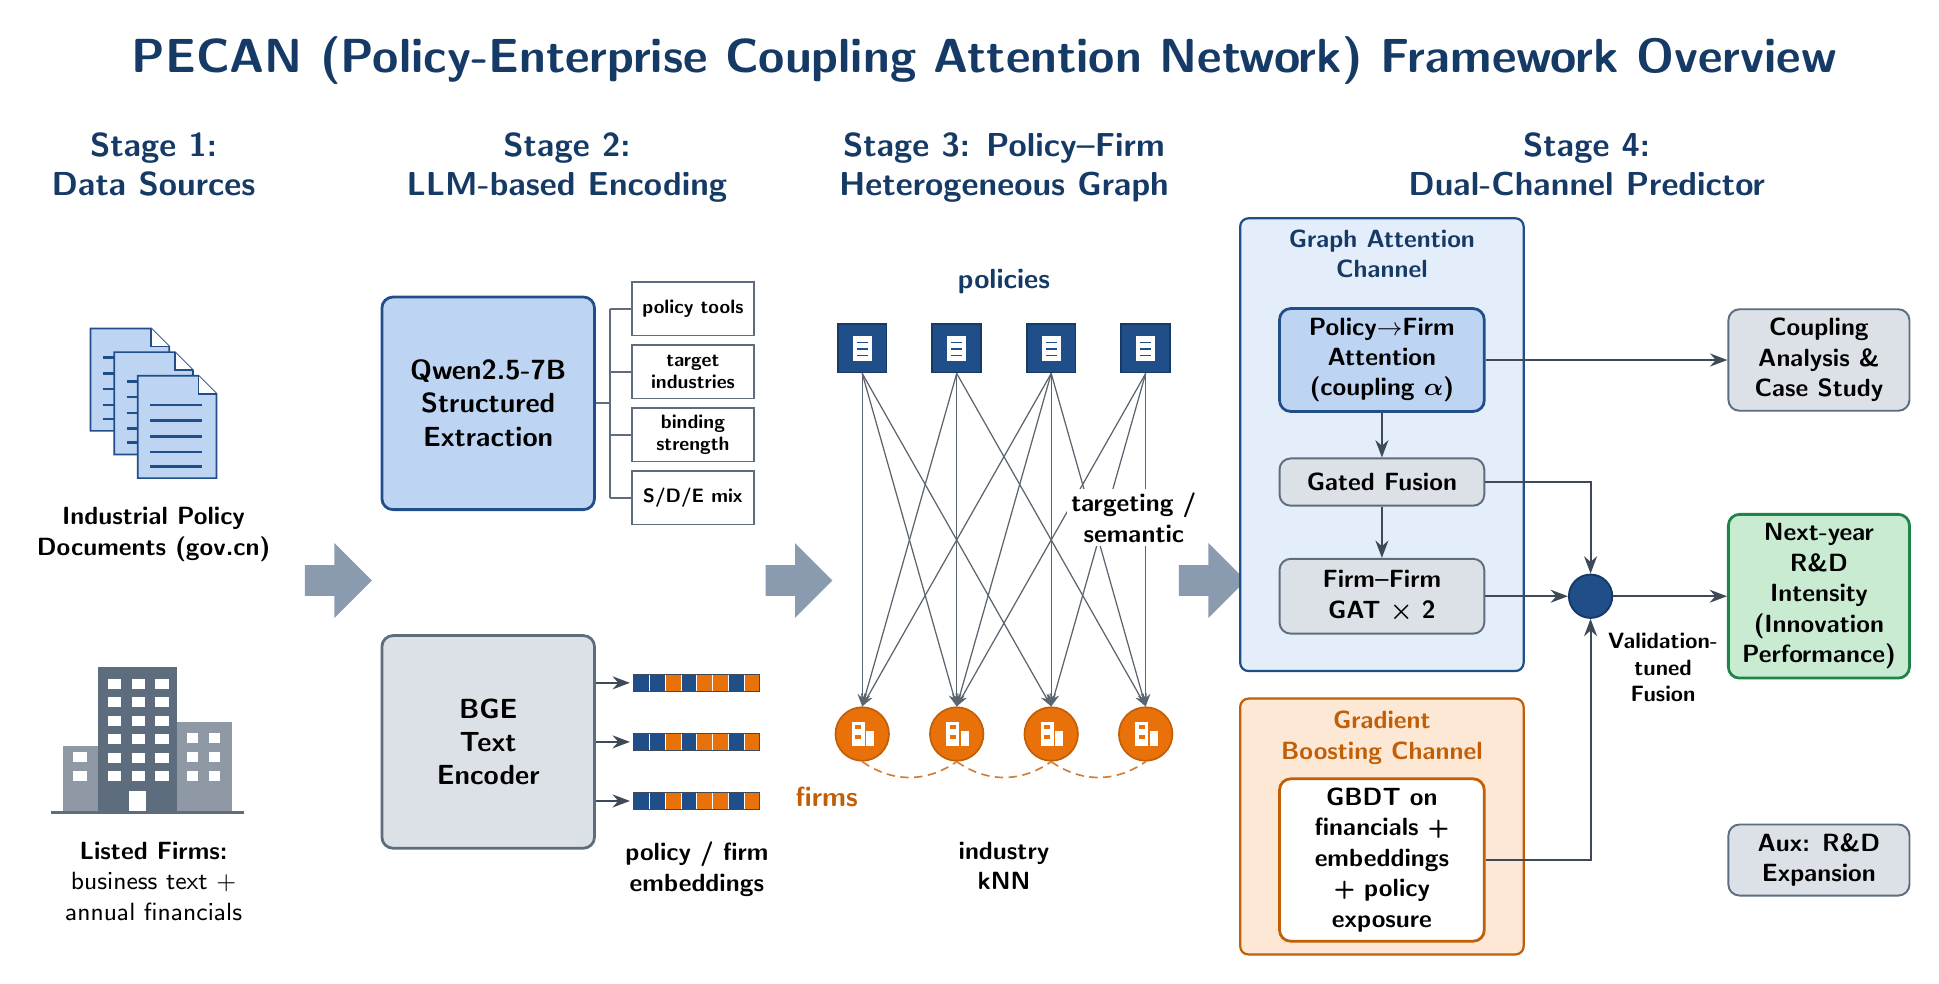
\begin{tikzpicture}

% ================= title =================
\node[font=\LARGE\bfseries, text=titleColor] at (12.05,12.1)
  {PECAN (Policy-Enterprise Coupling Attention Network) Framework Overview};

% ================= stage titles =================
\node[stagetitle, anchor=north] at (1.5,11.3)  {Stage 1:\\Data Sources};
\node[stagetitle, anchor=north] at (6.75,11.3)  {Stage 2:\\LLM-based Encoding};
\node[stagetitle, anchor=north] at (12.3,11.3){Stage 3: Policy--Firm\\Heterogeneous Graph};
\node[stagetitle, anchor=north] at (19.7,11.3) {Stage 4:\\Dual-Channel Predictor};

% ================= Stage 1 =================
\docicon{1.2}{8.05}
\docicon{1.5}{7.75}
\docicon{1.8}{7.45}
\node[lbl, anchor=north] at (1.5,6.55) {Industrial Policy\\Documents (gov.cn)};

\buildingicon{1.55}{3.45}
\node[lbl, anchor=north] at (1.5,2.3) {Listed Firms:\\\mdseries business text +\\\mdseries annual financials};

% ================= chevrons =================
\node[chevron] at (3.75,5.5) {};
\node[chevron] at (9.6,5.5) {};
\node[chevron] at (14.85,5.5) {};

% ================= Stage 2 =================
\node[box=blueLine, fill=blueFill, line width=1pt, minimum width=2.7cm, minimum height=2.7cm,
      font=\normalsize\bfseries] (qwen) at (5.75,7.75)
  {Qwen2.5-7B\\Structured\\Extraction};
\node[tag] (t1) at (8.35,8.95) {policy tools};
\node[tag] (t2) at (8.35,8.15)  {target\\industries};
\node[tag] (t3) at (8.35,7.35)  {binding\\strength};
\node[tag] (t4) at (8.35,6.55) {S/D/E mix};
\draw[grayLine, line width=0.6pt] (qwen.east) -- (7.3,7.75);
\draw[grayLine, line width=0.6pt] (7.3,8.95) -- (7.3,6.55);
\foreach \t in {t1,t2,t3,t4} \draw[grayLine, line width=0.6pt] (7.3,0 |- \t.west) -- (\t.west);

\node[box=grayLine, fill=grayFill, line width=1pt, minimum width=2.7cm, minimum height=2.7cm,
      font=\normalsize\bfseries] (bge) at (5.75,3.45)
  {BGE\\Text\\Encoder};
\embbar{7.6}{4.2}
\embbar{7.6}{3.45}
\embbar{7.6}{2.7}
\foreach \y in {4.2,3.45,2.7} \draw[arr] (bge.east |- 0,\y) -- (7.55,\y);
\node[lbl, anchor=north] at (8.4,2.3) {policy / firm\\embeddings};

% ================= Stage 3 =================
\node[font=\normalsize\bfseries, text=blueDark] at (12.3,9.3) {policies};
\foreach \i/\x in {1/10.5,2/11.7,3/12.9,4/14.1}{
  \node[draw=blueDark, fill=embBlue, minimum size=0.62cm, inner sep=0pt,
        line width=0.6pt] (p\i) at (\x,8.45) {};
  \fill[white] ($(p\i)+(-0.12,-0.16)$) rectangle ($(p\i)+(0.12,0.16)$);
  \foreach \yy in {0.07,-0.01,-0.09} \draw[embBlue, line width=0.4pt]
     ($(p\i)+(-0.07,\yy)$) -- ($(p\i)+(0.07,\yy)$);
  \node[circle, draw=orangeLine, fill=orangeFill, minimum size=0.68cm,
        line width=0.6pt] (f\i) at (\x,3.55) {};
  \fill[white] ($(f\i)+(-0.13,-0.15)$) rectangle ($(f\i)+(0.03,0.15)$);
  \fill[white] ($(f\i)+(0.05,-0.15)$) rectangle ($(f\i)+(0.15,0.04)$);
  \foreach \yy in {0.06,-0.06} \fill[orangeFill] ($(f\i)+(-0.09,\yy)$) rectangle ++(0.08,0.05);
}
\foreach \a/\b in {1/1,1/2,1/3,2/1,2/2,2/4,3/1,3/2,3/3,3/4,4/2,4/3,4/4}
  \draw[edge] (p\a.south) -- (f\b.north);
\node[font=\small\bfseries, fill=white, inner sep=1.5pt, align=center] at (13.95,6.3) {targeting /\\semantic};
\node[font=\normalsize\bfseries, text=orangeLine] at (10.05,2.75) {firms};
\draw[densely dashed, orangeLine!80, line width=0.6pt] (f1.south) to[bend right=35] (f2.south);
\draw[densely dashed, orangeLine!80, line width=0.6pt] (f2.south) to[bend right=35] (f3.south);
\draw[densely dashed, orangeLine!80, line width=0.6pt] (f3.south) to[bend right=35] (f4.south);
\node[font=\small\bfseries, align=center, anchor=north] at (12.3,2.3) {industry\\kNN};

% ================= Stage 4 =================
% graph attention channel panel
\filldraw[fill=bluePanel, draw=blueLine, line width=0.8pt, rounded corners=3pt] (15.3,4.35) rectangle (18.9,10.1);
\node[font=\small\bfseries, align=center, text=blueDark] at (17.1,9.65) {Graph Attention\\Channel};
\node[box=blueLine, fill=blueFill, minimum width=2.6cm, minimum height=1.25cm, line width=1pt] (att)
  at (17.1,8.3) {Policy$\to$Firm\\Attention\\(coupling $\boldsymbol{\alpha}$)};
\node[box=grayLine, fill=grayFill, minimum width=2.6cm, minimum height=0.6cm] (gate)
  at (17.1,6.75) {Gated Fusion};
\node[box=grayLine, fill=grayFill, minimum width=2.6cm, minimum height=0.95cm] (ffgat)
  at (17.1,5.3) {Firm--Firm\\GAT $\boldsymbol{\times}$ 2};
\draw[arr] (att) -- (gate);
\draw[arr] (gate) -- (ffgat);

% gradient boosting channel panel
\filldraw[fill=orangePanel, draw=orangeLine, line width=0.8pt, rounded corners=3pt] (15.3,0.75) rectangle (18.9,4.0);
\node[font=\small\bfseries, align=center, text=orangeLine] at (17.1,3.5) {Gradient\\Boosting Channel};
\node[box=orangeLine, fill=white, line width=1pt, minimum width=2.6cm, minimum height=1.55cm] (gbdt)
  at (17.1,1.95) {GBDT on\\financials +\\embeddings\\+ policy\\exposure};

% coupling analysis
\node[box=grayLine, fill=grayFill, minimum width=2.3cm, minimum height=1.25cm] (coup)
  at (22.65,8.3) {Coupling\\Analysis \&\\Case Study};
\draw[arr] (att.east) -- (coup.west);

% fusion
\node[circle, draw=blueDark, fill=blueLine, minimum size=0.55cm, line width=0.7pt] (fus)
  at (19.75,5.3) {};
\draw[arr] (gate.east) -- (19.75,6.75) -- (fus.north);
\draw[arr] (ffgat.east) -- (fus.west);
\draw[arr] (gbdt.east) -| (fus.south);
\node[font=\footnotesize\bfseries, align=center, anchor=north west] at (19.85,4.95) {Validation-\\tuned\\Fusion};

% output
\node[box=greenLine, fill=greenFill, font=\small\bfseries, minimum width=2.3cm, minimum height=1.6cm,
      line width=1pt] (out) at (22.65,5.3) {Next-year\\R\&D\\Intensity\\(Innovation\\Performance)};
\draw[arr] (fus.east) -- (out.west);

\node[box=grayLine, fill=grayFill, minimum width=2.3cm, minimum height=0.85cm] (aux)
  at (22.65,1.95) {Aux: R\&D\\Expansion};

\end{tikzpicture}
\end{document}
